\documentclass[a4paper,twoside]{scrbook}
\usepackage{CJKutf8}
\usepackage{url}
\usepackage{biblatex}
\usepackage[colorlinks,linkcolor=red]{hyperref}
\usepackage{graphicx}
\addbibresource{v1pc.bib}
\begin{document}
\begin{CJK}{UTF8}{gbsn}
\title{Volume 1, Part C: Early Memory Model}
\author{EDI}

\frontmatter
\maketitle
\tableofcontents
\mainmatter

\chapter{Introduction}
\section{Collective Communications Library}
\subsection{NVIDIA Collective Communications Library(NCCL)}
1991年,Argonne 国家实验室、Cornell 大学、MIT、Oak Ridge 国家实验室和 Wisconsin 大学联合成立了 MPI 论坛\cite{mpiforum},旨在制定一个标准化的消息传递接口。1994 年,MPI 论坛发布了第一个 MPI 标准版本 1.0,该版本定义了 120 个函数,涵盖了点对点通信、集合通信、进程管理、数据类型操作和错误处理等功能。MPI不受任何主要标准机构的认可,但是它已成为对在分布式内存系统上运行的并行程序进行建模的进程之间通信的事实标准。随着并行计算需求的不断扩大,MPI不断演进至今已经发布了MPI 4.1版本。

2016年,NVIDIA研究员Nathan Luehr发现在实践中,多GPU环境下并行计算的效率并没有像理论分析的那样获得显著提升,原因是多GPU环境下处理器的利用率低以及处理器的数据交换占据了大量的计算时间。为了充分利用GPU间的带宽,Nathan Luehr提出了NVIDIA Collective Communications Library(NCCL)]\cite{nccl2016},NCCL是一个通信原语库,具备拓扑感知,构造了基于环的消息通知路径。对于连接在同一个PCIe总线上的GPU,NCCL可以很好地促进GPU带宽的利用,从而使得小部分的线程通信和大部分的线程计算能够同时进行。不过,NCCL只适用于单节点环境,虽然对于单节点内的GPU数量没有限制,但是对于混用不同型号的GPU处理效果不好。

2016年,A. A. Awan\cite{awan2016}等人针对高性能数据分析 (HPDA) 和深度学习 (DL) 等新兴应用对高性能计算 (HPC) 平台和编程框架的挑战,提出了一种高效的 MPI\_Bcast设计,用于在多 GPU 节点之间进行大规模 GPU 缓冲区通信,同时利用NCCL库高效地进行节点内地通信。实验结果表明,与现有的 MVAPICH2-GDR 实现相比,所提出的分层 MPI\_Bcast 设计可以将 CNTK 框架的训练时间提高高达 47\%。不过,该算法依赖于 NCCL 库和 MVAPICH2-GDR 运行时。这意味着算法只能在支持这些组件的系统上运行。对于不支持 NCCL 库或 MVAPICH2-GDR 运行时的系统,需要寻找其他方法来实现高效的大规模 GPU 通信。

2018年,Iman Faraji\cite{cpe4667}等人讨论了在MPI中进行GPU集体通信的优化方法,为了将GPU感知引入MPI集体通信,提出了GPU共享缓冲区感知(GSB)算法和二叉树(BTB)算法。设计了用于多GPU节点的分层框架,并将其用于(1) intra-node intra-GPU、(2) intra-node inter-GPU、(3) inter-node inter-GPU。在单GPU节点中,作者通过GSB和BTB来最小化集体通信中消息的大小,利用GPU共享缓冲区和CUDA进程间通信支持MPI进程之间的GPU通信。在多GPU节点中,作者组合GSB—BTB算法,结合MVAPICH2进行全局操作提高集体通信性能。
\subsection{Microsoft Collective Communication Language(MSCCLang)}
2023年,Aashaka Shah\cite{shah2023taccl}等人提出opology Aware Col-lective Communication Library(TACCL)。针对不同拓扑结构需要重新单独设计算法的问题,TACCL引入了通信草图概念,包含逻辑拓扑、交换机超边策略、算法对称性和输入大小等信息,允许算法设计师只考虑顶层设计而不用实施底层实现。相比于NCCL,TACCL在多个集合通信操作和硬件拓扑上都展现出了优势,比NCCL快1.7-6。7不等。

2023年,Meghan Cowan\cite{cowan2023mscclang}等人提出了Microsoft Collective Communication Language(MSCCLang),旨在解决大规模机器学习模型在多 GPU 系统上训练和推理时,集体通信成为瓶颈的问题。它包含一个领域特定语言(DSL)用于编写集体通信算法,以及一个优化编译器,将算法转换为可执行的代码,并能够在基于解释器的运行时环境中高效灵活地执行。
\section{Remote Procedure Call}
本章节参考了\href{https://cloud.tencent.com/developer/article/1619589}{RPC发展史}

这里提及的远程过程调用(Remote Procedure Call,RPC)是广义上远程调用手段,是一种允许两个实体通过通用请求/响应机制的通信通道进行通信的设计范例,包括RPC(remote procedure call,远程过程调用)、SOAP(simple object access protoal,简单对象访问协议)、REST(representational state transfer,表达性状态转移)等设计范例。

1984年,Birrell\cite{birrell1984implementing}等人在《Implementing remote procedure calls》中对RPC做了最经典的解释。作者阐述了RPC传输协议的设计目标,描述了简单调用、复杂调用、异常处理、性能优化等问题,如图\ref{fig:A simple call}所示,文章给出了一次调用的实例图,用户代码通过本地调用请求 RPC,将参数传递给用户存根。用户存根将参数打包成调用数据包,并将其发送给 RPC 运行时。RPC 运行时负责将调用数据包可靠地传输到被调用方机器。
\begin{figure}[!htbp]
\centering
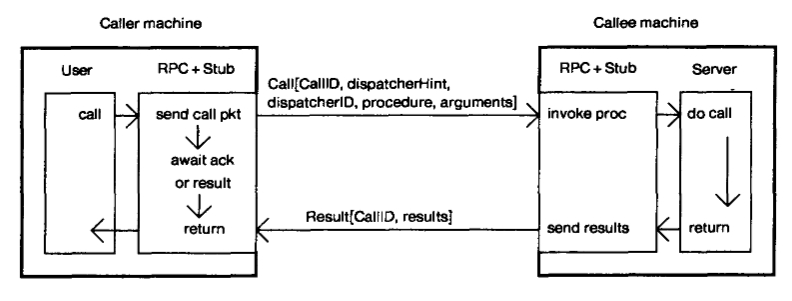
\includegraphics[width=1\textwidth]{Figures/A simple call.png}
\caption{一次调用过程} 
\label{fig:A simple call}
\end{figure}
1988年,RFC 1057 发布,ONC RPC 被定义为标准的RPC 规范,ONC RPC 提供了一个编译器,需要一个远程过程接口的定义来生成客户端和服务器的存根函数。这个编译器叫做 rpcgen。在运行此编译器之前,程序员必须提供接口定义。包含函数声明的接口定义,通过版本号进行分组,并被一个独特的程序编码来标识。该程序编码能够让客户来确定所需的接口。版本号是非常有用的,即使客户没有更新到最新的代码仍然可以连接到一个新的服务器,只要该服务器还支持旧接口。
\subsection{Common Object Request Broker Architecture(CORBA)}
分布式计算与面向对象编程的结合催生了分布式对象中间件,OMG在此需求的基础上提出了CORBA。CORBA是面向对象的应用程序体系规范,为用户提供接口定义语言(IDL)来指定远程对象类接口。用户的请求以对象代理请求(ORB)的方式处理,ORB截取客户发送的请求,并负责在该软件总线上找到实现该请求的服务对象,然后完成参数、方法调用,并返回最终结果。自OMG提出CORBA之后,CORBA经过了一段时间的黄金期,但是还是因为各种因素逐渐退出了历史舞台。下文详细分析了CORBA经历的早期发展、中期挑战、后期衰落以及发展现状等内容\cite{siegel1998omg} \cite{henning2006rise}。

(1)早期发展 (上世纪90年代初):1991年, OMG提出了CORBA1.0,用于帮助开发人员构建异构分布式应用。CORBA为用户提供了 IDL (接口定义语言),用于定义对象接口的标准语言,确保不同编程语言之间的互操作性;ORB (对象请求代理),管理对象调用和通信,隐藏底层细节,简化开发;IIOP (互联网ORB协议),标准的网络通信协议,确保跨网络传输的互操作性。得益于其强大的互操作性、成熟的分布式计算模型、丰富的标准服务以及广泛的应用成功案例,使其成为构建大型企业级应用的首选技术之一。

(2)中期挑战 (上世纪90年代中后期):1996年,添加了几个主要功能,包括用于客户端可移植性扩展的动态骨架接口(动态调用的镜像),初始参考解析器到接口库“开箱即用”互操作体系结构(GIOP、IIOP®、DCE-CIOP),支持COBOL的分层安全和事务服务数据类型扩展、科学处理、与OLE2/COM的宽字符互操作。OMG发布CORBA2.0,不过,CORBA2.0的推广并不顺利,Java 和 Web 开始兴起,虽然CORBA提供了Java语言映射,但是并没有涉及到爆炸式增长的Web。商业公司并没有等待CORBA给出解决方案,它们转向了其它技术,并且开始构建他们基于Web浏览器、HTTP、Java和EJB的电子商务基础设施。

(3)后期衰落 (2000年初): 2000年初,互联网泡沫破裂,XML 和 Web 服务兴起,进一步削弱 CORBA 的市场地位。CORBA的衰落是有原因的,可以分为技术上的复杂性和组织流程上的失败。
技术问题:

API的复杂性: API 复杂且难以使用,架构选择不当,类型系统过于庞大。

安全功能不足: 缺乏安全性和版本控制机制。

其他技术问题: 互操作性协议设计缺陷,编码冗余,缺乏对线程和异步调用的支持等。

上述的技术问题带来的结果就是,CORBA学习曲线陡峭,技术复杂,不容易正确使用,这些因素导致开发周期长、易出错。早期的实现常常充满Bug并且缺乏有质量的文档,有经验的CORBA程序员稀缺。

流程问题:

OMG是一个基于成员一致同意来发布技术的组织。从根本上来说,成员通过投票来将意见征求书变成规范。成员公司提交草案规范作为回应,OMG的成员们通过投票来决定是否将提案接受为标准。理论上,这是一个民主、公平的过程,但是实际上,它并不能起作用。标准化过程中没有什么准入资格。一些贡献者是领域专家,但是,令人感到挫折的是,大量的成员几乎不理解他们所要投票的技术,并且参与投票的厂商之间存在利益冲突。

缺乏对现有最佳实践的标准化,以及对参考实现和实际应用项目的需求,导致技术不成熟和难以使用。

(4)现状: CORBA 主要用于企业内部网络和实时嵌入式系统开发,已沦为垂直领域的细分技术。

\subsection{XML-RPC}
SOAP是一种建立在XML上的通信协议。

1998 年 XML 1.0 发布,被 W3C (World Wide Web Consortium) 推荐为标准的描述语言。同年,微软和DevelopMentor发布SOAP(Simple Object Access Protocol),随后提交给W3C作为标准。SOAP是一个严格定义的信息交换协议,使用XML作为RPC新的对象序列化机制,用于在Web Service中把远程调用和返回封装成机器可读的格式化数据。SOAP 的服务发现用的是 UDDI(Universal Description, Discovery, Integration) 统一描述发现集成,相当于一个注册中心,服务提供方将 WSDL 文件发布到注册中心,使用方可以到这个注册中心查找。

SOAP严格意义上是属于XML-RPC(XML Remote Procedure Call)技术的一个变种,一个XML-RPC请求消息就是一个HTTP-POST请求消息,其请求消息主体基于XML格式。客户端发送XML-RPC请求消息到服务端,调用服务端的远程方法并在服务端上运行远程方法。远程方法执行完毕后返回响应消息给客户端,其响应消息主体同样基于XML格式。远程方法的参数支持数字、字符串、日期等,也支持列表数组和其他复杂结构类型,SOAP是第一次真正成功地解决了多语言多平台支持的开放性RPC标准。
\subsection{RESTful API}
Restful是一种基于HTTP的架构设计风格。

2000年,Roy Thomas Fielding在《Architectural Styles and the Design of Network-based Software Architectures》\cite{fielding2000architectural}中首次提出了REST架构,直到目前仍然是Web开发的主流架构设计风格。REST架构风格定义了六个指导性约束。
\subsubsection{客户端-服务器架构}
通过将用户界面问题与数据存储问题分开,提高了跨多个平台的用户界面的可移植性,并通过简化服务器组件提高了可扩展性。
\subsubsection{统一接口}
统一接口是一切 RESTful Web 服务设计的基础。其表示服务器以标准格式传输信息。格式化的资源在 REST 中称为表征。此格式可以与服务器应用程序上资源的内部表征不同。例如,服务器可以将数据存储为文本,但以 HTML 表征格式发送该数据。

统一接口强制实施四个架构约束:

(1)请求应确定资源,它们通过使用统一的资源标识符实现此功能。

(2)客户端包含资源表征中的足够信息以修改或删除资源(如需要),服务器通过发送进一步描述资源的元数据以符合这一条件。

(3)客户端接收有关如何进一步处理表征的信息,服务器通过发送自描述信息实现此功能,该信息包含了有关客户端如何以最佳方式使用这些信息的元数据。

(4)客户端接收有关其完成任务需要的所有其他相关资源的信息,服务器通过在表征中发送超链接实现此功能,以便客户端可以动态发现更多资源。
\subsubsection{无状态}
在 REST 架构中,无状态指一种服务器独立于所有之前的请求完成每个客户端请求的通信方法。客户端可以以任意顺序请求资源,每个请求为无状态或与独立于其他请求。此 REST API 设计约束意味着服务器每次可以完全识别和满足请求。 
\subsubsection{层次化系统}
在层次化系统架构中,客户端可以连接到客户端和服务器之间的其他授权中间方,其仍将接收来自服务器的响应。服务器也可以将请求传递到其他服务器。您可以将 RESTful Web 服务设计为在包含多个层级(例如安全、应用程序和业务逻辑)的数个服务器上运行,从而共同满足客户端请求。这些层级对客户端仍不可见。
\subsubsection{高速缓存能力}
RESTful Web 服务支持缓存,缓存是指将一些响应存储在客户端或中间方上以提高服务器响应时间的流程。例如,假设您访问某个网站,该网站的每个页面都包含通用的页眉和页脚图像。每次您访问新的网站页面时,服务器必须重新发送相同的图像。为了避免出现这种情况,客户端在首次响应后会缓存或存储这些图像,之后直接使用缓存中的图像。RESTful Web 服务通过使用自行定义为可缓存或不可缓存的 API 响应来控制缓存。
\subsubsection{按需编码}
在 REST 架构风格中,服务器可以通过将软件编程代码传输到客户端暂时扩展或自定义客户端功能。例如,当您在任何网站上填写注册表单时,浏览器会立即高亮您填写内容的任何错误,例如不正确的电话号码。正是由于服务器发送的代码,浏览器才可以实现这个功能。
\subsection{微服务架构}
随着互联网数据的指数式增长,微服务架构开始出现并普及,分布式系统开始变的无处不在,REST架构的缺点开始显现,基于JSON或者XML 的消息冗余严重,导致性能下降。

2008年,Google 开源 Protocol Buffer,这是一种轻便高效的结构化数据存储格式,可以用于结构化数据序列化,很适合做数据存储或 RPC 数据交换格式。它可用于通讯协议、数据存储等领域的语言无关、平台无关、可扩展的序列化结构数据格式。

2008年,FaceBook 开源 thrift,这是一个跨语言的服务部署框架,最初由Facebook于2007年开发,2008年进入Apache开源项目。Thrift通过一个中间语言(IDL, 接口定义语言)来定义RPC的接口和数据类型,然后通过一个编译器生成不同语言的代码(目前支持C++,Java, Python, PHP, Ruby, Erlang, Perl, Haskell, C\#, Cocoa, Smalltalk和OCaml),并由生成的代码负责RPC协议层和传输层的实现。

2010年,Avro脱离Hadoop项目,成为Apache顶级项目。这是一个基于二进制数据传输高性能的中间件。在Hadoop的其他项目中例如HBase(Ref)和Hive(Ref)的Client端与服务端的数据传输也采用了这个工具。Avro 可以将数据结构或对象转化成便于存储或传输的格式。

2015年,Google 开源Google Remote Procedure Cal(gRPC),gRPC 使用 PB 作为序列化的解决方案,而在传输的介质上使用了 HTTP/2而不是常见的TCP。gRPC 是一个多路复用、双向流式 RPC 协议。在一般的 RPC 机制中,客户端发起到服务器的连接,只有客户端可以请求,而服务器只能响应传入的请求。然而,在双向 gRPC 流中,虽然初始连接是由客户端发起的(称为端点1) ,但是一旦建立连接,服务器(称为端点2)和端点1都可以发送请求和接收响应。这极大地简化了两个端点相互通信的开发(如网格计算)。由于两个数据流都是独立的,这也省去了在端点之间创建两个独立连接的麻烦(一个从端点1到端点2,另一个从端点2到端点1)。

\section{Consensus Mechanism}
\subsection{Classification of consensus mechanisms}
\subsubsection{Byzantine fault-tolerant(BFT)}
BFT自20世纪80年代提出以来\cite{lamport1982byzantine},已经得到了广泛的研究。在第一个被称为PBFT\cite{castro2002practical}的实用BFT协议之后,有许多实用BFT协议被提出。根据时序假设,BFT可以分为三种类型:同步、异步和部分同步协议。

2016年,Andrew Miller等人提出了HoneyBadgerBFT\cite{miller2016honey},这是第一个实用的异步BFT协议,它在不做任何时序假设的情况下保证了生存性。HoneyBadgerBFT的核心部分由两部分组成,分别是原子广播(Atomic Broadcast)和异步公共子集协议(Asynchronous Common Subset),在协议开始以前,每个主机准备好各自的提案(即试图写入共识的数据),启动N个原子广播的实例(N为网络中主机的个数)。在某一个原子广播完成以后遂将该广播对应的主机编号作为输入启动异步公共子集协议。异步公共子集协议在收集到足够多的主机编号后终止,所有的非敌手主机得到一个关于子集的共识。根据这个子集这些主机将从原子广播阶段获得的提案写入共识。

2017年,Yossi Gilad\cite{gilad2017algorand}等人在针对 PBFT 算法在很多节点情况下性能不佳的问题,提出先选出少量记账节点,然后再利用可验证随机函数(Verifiable Random Function,VRF)来随机选取领导节点,避免全网直接做共识,将拜占庭算法扩展到了支持较大规模的应用场景,同时保持较好的性能(1000+ tps)。

同年,Rafael Pass \cite{pass2017sleepy}等人探讨了在动态场景(大量节点离线情况)下如何保障共识的安全性,提出的 Sleepy Consensus 算法可以在活跃诚实节点达到一半以上时确保完成拜占庭共识。

2019年,Maofan Yin 等在论文《HotStuff: BFT Consensus with Linearity and Responsiveness》\cite{yin2019hotstuff}中对 PBFT 算法进行了改进:利用主节点来简化通信量,同时将视图切换与共识操作进行统一。值得一提的是,Facebook Libra 白皮书中采用了该成果。

\subsubsection{Consensus mechanism based on proof of concepts}
由于无许可的区块链网络不允许身份验证或显式同步方案。因此,期望其中的共识协议具有良好的可扩展性,并且能够容忍伪身份和较差的同步。由于任何节点都能够为区块链头部提出具有自己的候选块的状态转换,因此无许可网络中的共识协议的主要目标是确保每个共识节点都遵守“最长链规则”[3]。也就是说,当块被组织在链表中时,在任何时间实例中,只有最长的链可以被接受为区块链的规范状态。由于缺乏身份验证,基于直接投票的BFT协议不适合无许可的区块链网络。基于激励的Nakamoto Consensus\cite{nakamoto2008bitcoin}被广泛采用。

在Nakamoto Consensus的基础下,产生了许多基于概念证明的共识机制,包括PoW、
PoUS、uPoW、PoR、PoST、PoM、PoH等方案。

\subsubsection{Virtual Block Mining and Hybrid Consensus Mechanisms Beyond Proof of Concept}
2019年,Wenbo Wang等人在《A Survey on Consensus Mechanisms and Mining Strategy Management in Blockchain Networks》\cite{wang2019survey}对超越概念证明的虚拟块挖掘和混合共识机制进行了讨论,文中提出了两种类型:基于权益证明和虚拟挖矿与混合共识协议。

在基于权益证明和虚拟挖矿中,介绍了PoS的概念,它是一种修改后的PoW方案,旨在减少因耗尽哈希查询而产生的能源消耗。讨论了纯PoS协议的设计,例如Ouroboros协议,它使用“跟随硬币”算法来选举区块提议的领导者,并根据持有者的股份进行随机分配。讨论了基于委员会的PoS协议,例如PoA和Snow White协议,它们将领导者选举和区块生成/验证过程结合在一起,类似于传统的拜占庭容错协议。

在混合共识协议中,讨论了将Nakamoto协议与快速拜占庭容错协议(如BFT)结合起来的方法,以实现更高的吞吐量和立即的最终性。介绍了Bitcoin-NG协议,它将共识过程分解为领导者选举和事务序列化两个平面,并使用两种类型的区块来实现更高的吞吐量。讨论了PeerCensus协议,它使用PoW方案来选择BFT委员会成员,并确保事务提交与区块生成独立进行。讨论了将虚拟挖矿机制(如PoS)与BFT协议结合起来的方法,例如Tendermint协议,它使用股份来衡量投票权,并通过轮询方案来选择区块提议的领导者。

\subsection{Analysis of Consensus Mechanisms}
FLP不可能原理表明:异步的分布式系统中不存在面向任意场景的共识算法。CAP原理表明:分布式系统最多只能同时满足一致性、可用性和分区容错性中的两项特性。因此在设计分布式系统时,设计完美的确定性分布式协议是徒劳无功的。但是,不同于传统的分布式系统,区块链网络是分布式和去中心化结合的网络,因此需要根据区块链网络的特点作出有别于传统分布式系统的CAP定义:
\begin{itemize}
\item[$\bullet$]一致性:分布式对等系统中的概率共识可以解决拜占庭故障,从而达到最终的一致性。
\item[$\bullet$]可用性:每次请求都能获取到非错的响应,但是不保证获取的数据为最新数据。
\item[$\bullet$]分区容忍性:系统能够在一定的时限内达成数据一致性。
\end{itemize}

为了满足实际应用场景的需求,区块链的共识协议需要在一致性、可用性和分区容忍性实现完美平衡。考虑到不同应用场景的差异,因此提出了几个重要的评价指标用于衡量不同的共识机制。
\begin{itemize}
\item[$\bullet$]共识机制的拜占庭容错能力
\item[$\bullet$]共识机制的去中心化水平
\item[$\bullet$]提案节点的选择机制
\item[$\bullet$]需要形成的共识内容
\item[$\bullet$]节点达成共识的形式
\item[$\bullet$]激励机制和惩罚机制
\item[$\bullet$]应对恶意攻击的能力
\end{itemize}

\subsubsection{BTC}
BTC是一个分布式对等账本。一个加入BTC网络的用户可以生产任意个成对的公钥和私钥。私钥由用户保存,是不应该泄露给他人的。私钥可以用于对消息签名,签名不可伪造,并且是可以通过私钥对应的公钥验证的。密码学保证签名具有以下特点:

(1)有效性。如果用户用私钥签名了一个消息,那么其他任何人使用私钥对应的公钥、消息原文来验证签名,该签名必须是有效的。

(2)不可伪造性。如果没有掌握某个私钥,就无法对一条之前该私钥没有签过名的消息生成一个签名,并且使它可以被公钥验证为有效。也就是说,仅仅掌握了公钥是无法伪造相应私钥的签名的。在实际情况中,找到公钥对应私钥的代价通常非常巨大,以至于我们认为这是“无法完成的”。

一次共识过程开始于节点对“哪些未确认的交易应该被确认”发出提案。在BTC网络中,交易都是被“打包”放进区块进行处理的。区块(Block)是一个精心设计的数据结构,它包含两部分。第一部分是一个哈希指针,它包含上一区块的哈希值,可以表明自己上一个区块的信息。第二部分是一个Merkle树,它的叶节点是被打包进该区块的所有交易的哈希值,非叶子节点则是根据它的两个子节点计算出的哈希值。通过Merkle各节点的哈希可以方便地验证该区块内所有交易的完整性。

一个区块还包含了一个coinbase交易(币基交易),这部分固定的奖励BTC是被新“创造”出来的,将被支付给打包这个区块的节点。节点的选择来源于节点之间有竞争“记账权”的动力,竞争过程所有的节点都可以参与,每个节点都希望自己打包的区块成为系统的长期共识(最终一致性共识),因为只有这样自己才能获得币基交易的奖励。记账权的确认来源于一个数字解谜过程,即寻找nonce的过程,谁最先找出对应的nonce谁就获得记账权。

通过采用最长链原则达成最终一致性,每个区块都包含有一个指向前一区块的哈希指针,并由此可以追溯到创世区块,我们定义从创世区块到这个区块所形成的“链”上的区块总数为该区块的区块高度。BTC网络规定,当网络中存在所谓的“分叉”时,即多个区块同时引用了同一个区块的哈希指针,只有最长链(即区块高度最高的链)上的交易会被承认,因此比特币的拜占庭容错能力是50\%。区块链没有设计直接的惩罚机制,但是违反最长链原则需要至少拥有全网算力的51\%,因此节点恶意行为不能影响大于50\%的网络就是无用功,白白浪费算力和资源,博弈论告诉我们,如果在短链上解谜的节点是理性的,那么它们应该立即抛弃这条较短的链,切换回最长链。因此,整个系统必然会在一个时刻,使所有接入网络的节点对系统的状态达成一致,所达成的共识就是当前的最长链。

\url{https://medium.com/@tokenroll/%E5%9D%8E%E5%9D%B7%E7%9A%84-%E5%85%B1%E8%AF%86%E6%9C%BA%E5%88%B6-%E4%B9%8B%E8%B7%AF-%E5%8C%BA%E5%9D%97%E9%93%BE%E6%8A%80%E6%9C%AF%E5%BC%95%E5%8D%B7%E4%B9%8B%E4%B8%80-25557c66af70}
\subsubsection{ETH2.0}
Gasper 是一个由信标链协议实现的抽象的权益证明协议层。在信标链协议中,参与的节点(或者叫 “验证者”)都在系统中存有保证金(stake,形式为 ETH)。验证者通过向网络提交见证消息(attestation) 来证实区块的有效性并为其多种属性投票。信标链协议本身包含了多种工具,以帮助验证者们对区块链的最新状态达成共识。

\begin{figure}[!htbp]
\centering
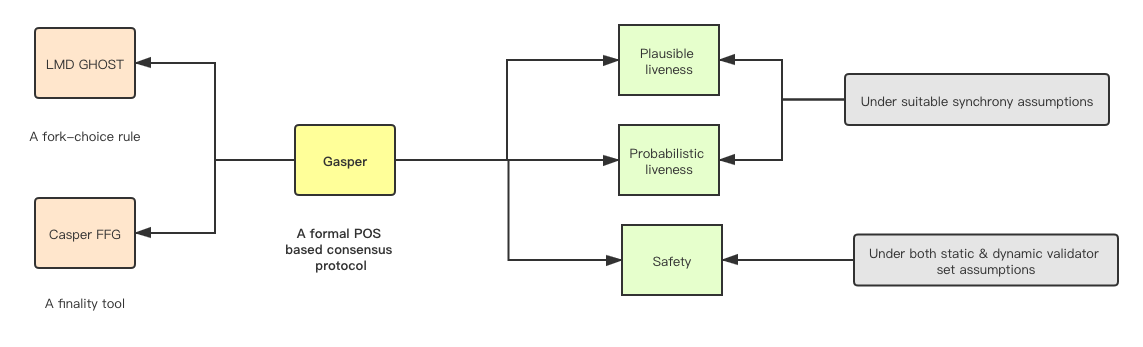
\includegraphics[width=1\textwidth]{Figures/read-gasper.png}
\caption{Gasper} 
\label{fig:Gasper}
\end{figure}

如图\ref{fig:Gasper}所示,Gasper 要解决的是Ethereum2.0 共识层的 Fork choice 和 block最终确定性(finality)的问题。Gasper 是Casper FFG 算法(Casper the Friendly Finality Gadget, 下文称Casper)和 LLMD GHOST(下文称GHOST) 的组合。 Casper解决的是finality, GHOST解决的是Fork choice。

Casper FFG 算法由Vitalik Buterin\cite{buterin2017casper}在2017年提出,Casper FFG在当前PoW的基础上,添加了一层PoS投票过程,进一步增强了Finality, 旧的区块理论上不可能被撤销。Casper FFG是一个没有侵入性的算法,它没有改变当前Ethereum的PoW算法,只是在这一层PoW上添加了BFT风格的PoS,也就是说所有的块,还是PoW矿工挖出来的,这条核心流程保留了下来。在这基础上,每挖出100个块,PoS的验证节点们会对最后一个块进行投票,2/3通过后,这最后一个块称为checkpoint(检查点)。凡是被finalized的检查点,不可撤销。总结一句话,就是保留了PoW出块的机制,同时每隔100个块来一次PoS投票,进一步增强了Ethereum的安全性(Safety,即Finality). 所有最终确定的检查点都成为规范链(区块链历史的一部分),所有忠诚节点都同意他们永远不会逆转这条链。「最终检查点」之后的区块可以随意分叉,但之前的区块不允许分叉。

LMD-GHOST(Latest Message Driven GHOST)由Yonatan Sompolinsky\cite{sompolinsky2015secure}在2015年提出,它是一种分叉选择的规则,主要用于处理pos中的分叉。其实在以太坊上一个版本中就提到过GHOST协议,用于产生分叉带来叔块引用,将此协议做了pos环境下的升级,依据投票比重来选择正确的区块。由于网络延迟或者潜在攻击的问题,新的区块产生可能会发生分叉,这时,我们选择的策略就叫LMD(最新的消息驱动),我们会选择票数最多(权重)的链作为权威链,这一点区分于pow中的最长链原则。如图\ref{fig:GHOST}所示, 圆圈表示validator, 方块表示block, block 中的数字表示区块上积累的投票数,子节点的投票会向上累加到父节点。 图中,蓝色区块为每一层上获得投票最多的区块,连在一起为当前视图中最可信的一条链。

\begin{figure}[!htbp]
\centering
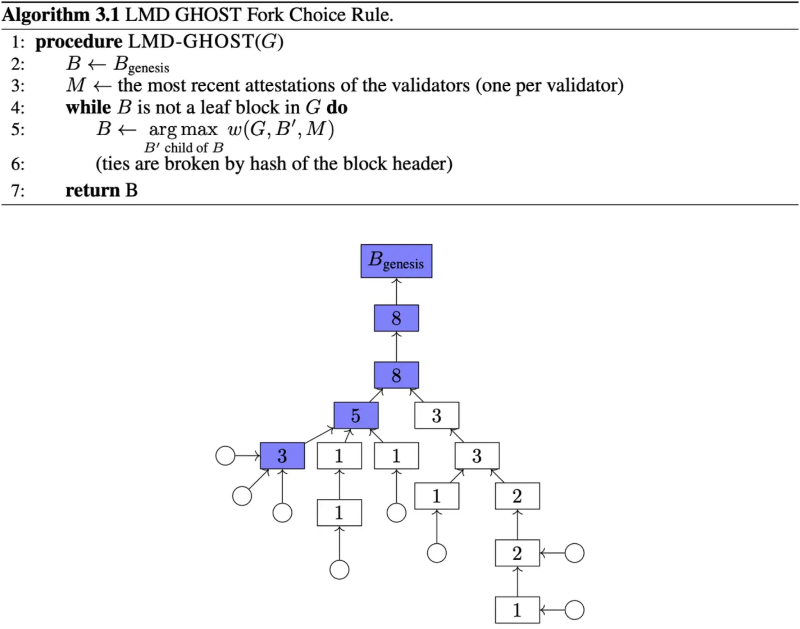
\includegraphics[width=1\textwidth]{Figures/GHOST.png}
\caption{LMD-GHOST} 
\label{fig:GHOST}
\end{figure}

为了更好的鼓励验证者诚信投票,pos针对投票设计了一套奖惩机制。奖励的组成如图\ref{fig:reward}所示,参与委员会,成为提议者,验证区块都可以获得奖励,其中,提议者的奖励是最多的,具体的比例和计算公式可从附录提供的资料查阅。

\begin{figure}[!htbp]
\centering
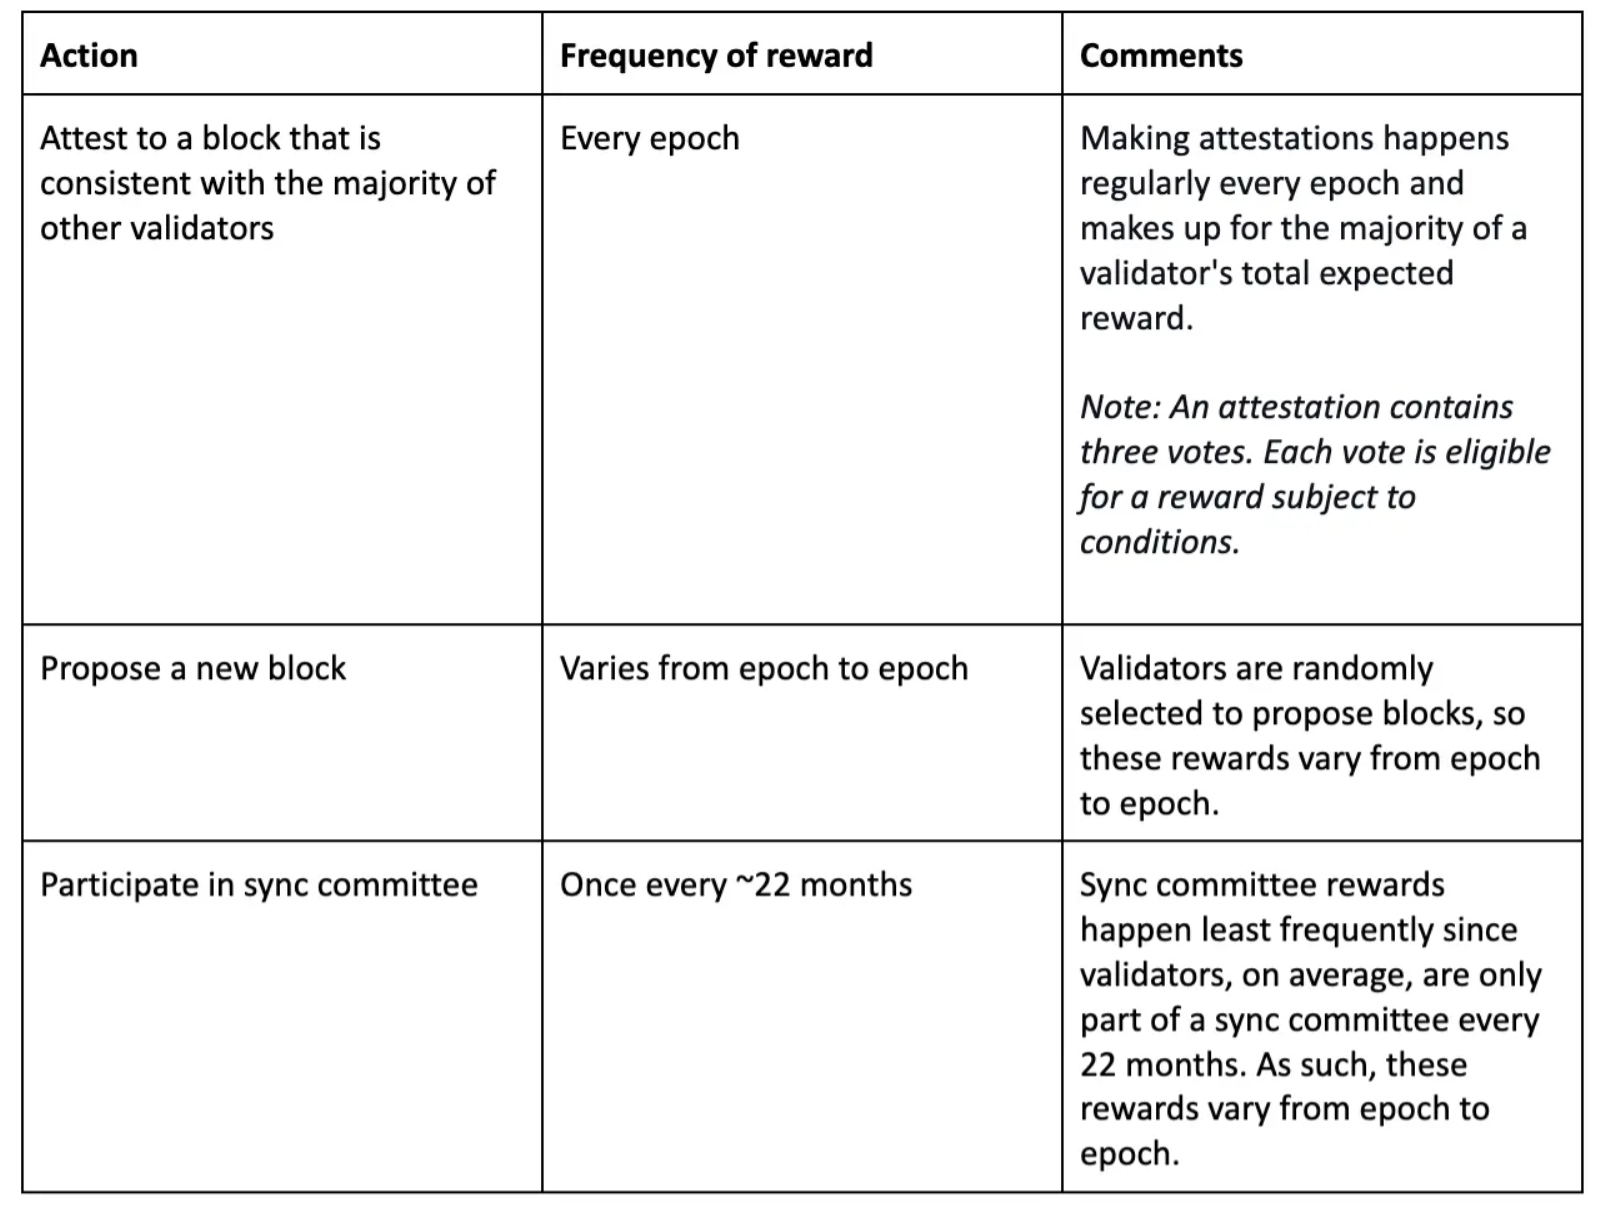
\includegraphics[width=1\textwidth]{Figures/eth reward.png}
\caption{ETH2.0 Rewards} 
\label{fig:reward}
\end{figure}

以太坊共识层面可能存在的攻击有很多种,这里主要介绍长程攻击(long range attacks),无利害攻击(noting to stake attacks)和大型质押攻击。

长程攻击有两种情况,第一种情况是,攻击者作为参与创始区块的验证者,在原本的区块链旁维护一个单独的区块链分叉,并最终说服诚实的验证者在很久以后的某个时间点切换过去。但是该攻击在信标链上无法实现,因为“finality gadget”可确保所有验证者定期就诚实链的状态(“检查点”)达成一致,此后检查点之后的区块将无法再进行重组。第二种情况是,当新节点加入网络时,将从离其最近的节点处获取信息(称为弱主观性检查点)作为伪创始区块构建区块链。**这将为加入网络的新节点创建一个“信任网关”,然后其才能开始自己验证区块。然而,从区块浏览器等客户端收集构建检查点所需的可信区块信息,并不能增加客户端本身的可信度,因此主观性是“弱的”。因为根据定义,检查点由网络上的所有节点共享,所以不诚实的检查点是共识失败的状态。

无利害攻击就是说相对于pow而言,pos分叉成本非常低,因为对于单个矿工来说,自身算力是有限的,所以为了利益它必须遵守最长链原则,而pos一旦获得投票资格,可以随意支持区块造成分叉所以才会有奖惩机制的设立,避免这种攻击行为。

大型质押攻击就是说攻击者持有相应比例的eth时,会触发以下危机:

33\%:延迟终局性

34\%:导致双重终局性

51\%:控制区块链的未来

66\%:控制区块链的过去

质押攻击主要的应对措施就是通过惩罚机制将攻击者强制退出网络,发起社区提议罚没攻击者资产,在现实社交网络进行协调等等。

ETH2.0采用的Gasper协议基于pBFT实现,因此和pBFT一样,具有1/3的拜占庭容错。

\url{https://learnblockchain.cn/article/4778#GHOST}

\url{https://learnblockchain.cn/article/6037#2.5%20pos%E5%A5%96%E6%83%A9}

\url{https://www.web3sj.com/news/21111/}

\subsubsection{Solana}
PoH 的核心是一种类似于可验证延迟函数 (VDF) 的简单哈希算法。 Solana 使用SHA-256来实现这一点,并使用一次迭代的输出作为下一次迭代的输入。该计算在每个验证器的单个核心上运行。虽然序列生成是顺序且单线程的,但可以并行验证输出,从而可以在多核系统上进行高效验证。这个机制允许 Solana 以加密的方式展示真实时间已经过去,生成连续的输出。因此,存在清晰、可验证的交易顺序,确保了一致的事件时间轴。验证者因此可以轻松验证经过的时间有多长,进一步增强了网络的可信度。篡改哈希链的任何部分都会需要重新计算所有后续的哈希,这是一项算力密集型的工作,可保护网络免受更改的影响。

PoH(历史证明)显著减少了验证者每个区块需要处理的信息量。通过使用交易最新状态的哈希版本,区块确认时间被大幅缩短。当验证者(或复制节点)收到一个区块时,PoH(历史证明)序列为它们提供了一个具有加密可靠的交易顺序,他们可以在无需重新验证的情况下信任。这种效率对于加快共识机制至关重要,因为网络可以迅速选择并转移到下一个验证者进行区块验证。

Solana使用结合PoH和Tower BFT的共识机制,在碎片(部分区块)传播到其他验证器后运行。Tower BFT是一种类似pBFT的共识算法,旨在利用PoH同步时钟运算,节省验证节点验证区块时间正确性的步骤。

在Solana的Tower BFT共识中,由两种角色参与。一种是领导者(区块生产者),另一种是验证者。领导者就是负责记录数据(或记账)的,而验证者则是负责对数据(或交易信息)进行验证的。Solana每一个工作epoch被划分为若干时隙,而领导者也会被安排成为一个时间表,每个领导者在指定的时隙内工作。通俗地说,领导者们排好队,轮流出块。而验证者对区块信息进行确认。有超过2/3的验证者验证通过,就可以确认该区块的信息。

DBFT通过拜占庭容错算法来完成共识。DBFT共识算法具有1/3的容错性,只要有2/3以上的领导人达成共识,就可以完成出块。每一个区块都有最终性,不会产生分叉。另一方面,它使用了历史证明序列的方式来提速。在其他区块链中,某一个区块的确认出现了延迟,那这个区块其后的交易处理和数据存储都会延迟,必须要等到上一个区块信息确认完成以后,才可以继续后面的信息处理。而在Tower BFT算法中,验证者可以明确知晓下一个区块的领导者,那么当验证者收到新的交易信息以后,可以直接与下一个区块的验证者进行信息确认。也就是说,Solana中的出块和信息确认都是异步进行。记录一个块的信息,不需要等待上一个块的完成。

内存池管理(Gulf Stream),由于Solana使用了历史证明序列,每一个区块的信息在等待验证时形成了一个内存池。Solana的公链程序中会存储当前的领导者序时列表,用户也好、验证者也好,可以知晓下一个领导者是哪一个节点。因此,用户和验证者可以提前将交易转发给预期的领导者。换句话说,待处理的事务会流动到下一个区块的内存池中了。

历史证明序列的引入,改变了Solana的内存池结构。在其他公链上,所有的待确认信息处于同一个内存池,而在Solana由于信息在写入区块时,时间与信息会共同加密存储,这样信息的储存不会乱套,仍然可以分清谁先谁后。Solana每一个区块可以形成独立的内存池。解释是将事务缓存和转发推到网络边缘。事实上,是Solana是将确认的信息推到一个内存池的边界,流动到下一个区块的内存池之中,从而进行并行的处理。这使验证者可以提前执行事务,减少确认时间,更快地切换领导者,并减少来自未确认事务池的验证者的内存压力。

\url{https://steemit.com/sct/@tvb/solana}

\subsection{Tendermint}
Tendermint的节点分为两种类型:validator和非validator节点。validator节点参与共识,也就是对区块(包含一批交易)进行共识,包括propose区块,对提议的区块进行投票。而非validator节点不参与共识,但会帮助传播区块和投票消息,以及相互同步状态等。节点之间不一定两两相连,和一个节点直接相连的那些节点称作peers。无论是validator节点,还是非validator节点,都包含与共识过程相关的一些状态,如区块链当前高度height,round,以及step等。节点之间运行gossip协议,相互同步共识状态和区块链状态信息。

\begin{figure}[!htbp]
\centering
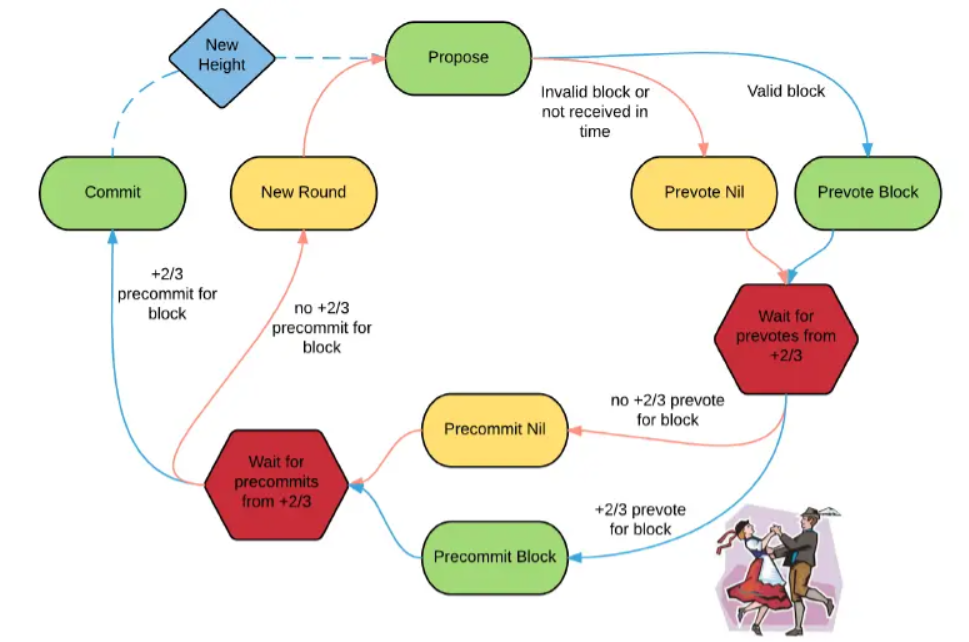
\includegraphics[width=1\textwidth]{Figures/Tendermint.png}
\caption{Tendermint} 
\label{fig:Tendermint}
\end{figure}

如图\ref{fig:Tendermint}描述了共识的过程:从Propose区块开始,进行Prevote和Precommit两个阶段的投票。如果投票达成共识,则依次进入Commit 和 NewHeight阶段,完成共识,区块链高度增加。整个过程称为一个round。不管投票是否达成共识,系统将推进到下一个round,进行新一轮的共识。

一个共识过程可能需要多个round的原因可能有:
(1)指定的proposer节点不在线。
(2)proposal block无效。
(3)节点没有及时收到proposal block。
(4)虽然proposal block有效,但是没有足够多的节点在Precommit 阶段及时收到对应的 +2/3 的prevotes。
(5)虽然proposal block有效,也有足够多的节点接收到了+2/3 的prevotes,但是没有足够多的节点收到+2/3 的 precommits。

类似上述情况的解决方法有:
(1)系统变更到下一个round,重新指定proposer节点。
(2)round变更时,增加各阶段的超时时间。

1、Propose 阶段(height:H,round:R)
在这一阶段,指定的proposer节点组装并广播proposal(提议内容)。
(1)proposer节点指定方式为:依据当前的round和各validator的投票权,采取确定性的、非阻塞的roundrobin选择算法来选取。

(2)proposal包含一个提议的区块,以及一个可选的、最新的PoLC-round(小于当前的round值R)。PoLC-round的含义是,针对该round,有一个PoLC,即有+2/3(多于2/3)的节点的prevote投票。仅在当前proposer节点知晓一个最新的PoLC-round时,才会将其包含在proposal中。 这里PoLC-round的作用是,必要时让节点从更旧的round 解除锁定,保持系统的liveness(活性)。

Propose 阶段结束条件为:
(1)超时时间内收到proposal block及PoLC-Round的所有prevote 投票(如果有的话),则立即转到下一阶段:Prevote(H,R);
(2)否则,等到timeoutProposeR超时, 转到下一阶段: Prevote(H,R)。这里可以看到,节点在Propose 阶段会等待一小段时间:timeoutProposeR,来接收proposal。这是Tendermint所基于的一个弱同步假设。除此之外,算法的其余步骤为异步的。

(3)公共退出条件
上述公共退出条件具体指的是:

收到针对特定block的 +2/3 的precommit 投票,则转到Commit(H)。

收到(H,R+x)的任何 +2/3 的 prevote 投票,则转到Prevote(H,R+x)。

收到(H,R+x)的任何 +2/3 的 precommit 投票,则转到Precommit(H,R+x)。

上述公共退出条件在接下来将介绍到的 Prevote 和Precommit 阶段也都会起作用。

2、Prevote 阶段 (height:H,round:R)

每个validator节点进入到Prevote 阶段后,会投prevote 投票并向其他节点广播其投票。首先,如果节点自LastLockRound起lock在某一block,此时却有PoLC-Round的、另一个block或nil的PoLC,则节点unlock。这里 LastLockRound < PoLC-Round < R;否则,如果节点还lock在某一block,则针对该block 进行prevote(投票并广播,之后所有类似表述都可以类比理解);
否则,如果proposed block有效,则对其prevote;否则,如果proposed block无效,或者 没有及时收到,则prevote nil。

Prevote 阶段的结束条件为:

(1)收到任何+2/3 的prevote 投票后等待一段时间:timeoutPrevote。如果该时间内收到针对一个特定block或nil的+2/3 的 prevote 投票,则立即转到下一阶段:Precommit(H,R);如果该时间内没有收到上述PoLC,则转到下一阶段:Precommit(H,R)。

3、Precommit 阶段 (height:H,round:R)

每个validator节点进入到Precommit 阶段后,会投 precommit 投票并广播其投票。
首先,在(H,R),如果节点有针对一个特定block的PoLC,则节点lock在该block,并且置LastLockRound =R,同时precommit 该block;否则,在(H,R),如果节点有针对 nil 的一个PoLC,则节点unlock,同时precommit nil;否则,节点将保持其目前的lock状态不变(即如果已经lock了,则继续lock,否则,继续保持unlock的状态) ,并且 precommit nil。

Precommit 阶段的结束条件为:

收到任何+2/3 的 precommit 投票后等待一段时间:timeoutPrecommit,如果该时间内收到针对nil的+2/3的precommit 投票,则相当于没有共识出有效区块,立即转Propose(H,R+1);否则,如果超时后也没有收到针对特定 block 的+2/3 的 precommit 投票,则相当于也没有共识出有效区块,转到Propose(H,R+1)。

4、Commit 阶段 (height:H)

这一个阶段中,节点尝试对区块进行commit:首先设置CommitTime = now()然后,节点等待接收完整的、将要 commit 的区块,然后转到 NewHeight(H+1) 阶段。

5、NewHeight 阶段 (height:H)

在这一阶段,节点最终完成整个共识过程的最后环节,使链的高度增加一个区块,具体步骤为:置LastCommit=Precommits(即+2/3的Precommit 投票的集合);增加区块高度,将共识出的新区块添加到链上;置StartTime = CommitTime+timeoutCommit;等待直到StartTime,以便接收延迟的commits.最后,转到 Propose(H,0),开始新的高度上的区块的共识。注意,此时round的编号又从0开始。

\url{https://juejin.cn/post/6844903973086822408}

\printbibliography
\end{CJK}
\end{document}
